\documentclass[conference]{IEEEtran}
\IEEEoverridecommandlockouts

\usepackage{cite}
\usepackage{amsmath,amssymb,amsfonts}
\usepackage{algorithmic}
\usepackage{graphicx}
\usepackage{textcomp}
\usepackage{xcolor}
\usepackage{hyperref}
\usepackage{url}

\def\BibTeX{{\rm B\kern-.05em{\sc i\kern-.025em b}\kern-.08em
    T\kern-.1667em\lower.7ex\hbox{E}\kern-.125emX}}

\begin{document}

\title{GraphRAG Approach to the NCA Encroach}

\author{\IEEEauthorblockN{Usaid Azeem}
\IEEEauthorblockA{\textit{Roll Number: 22i-0515} \\
\textit{Department of AI} \\
\textit{FAST-NUCES} \\
usaid.azeem@university.edu}
}

\maketitle

\begin{abstract}
This paper presents a comparative analysis between traditional Retrieval-Augmented Generation (RAG) and GraphRAG for global sensemaking tasks using UK National Crime Agency (NCA) documents. We implement both pipelines with controlled variables: same LLM (Mistral 7B), same dataset (155 NCA PDFs → 1,529 chunks), and same chunking strategy. Our GraphRAG approach uses rule-based entity extraction (deterministic, higher quality than LLM-based methods) to build a knowledge graph with 10,417 nodes and 32,806 edges, enhanced with semantic similarity edges, Louvain community detection, and K-Means cross-cluster bridges. Results show comparable response times (~7.2s) but superior global understanding for GraphRAG, validating its effectiveness for query-focused summarization tasks.
\end{abstract}

\begin{IEEEkeywords}
Retrieval-Augmented Generation, GraphRAG, Knowledge Graphs, Comparative Analysis, Crime Data Analytics
\end{IEEEkeywords}

\section{Introduction}
Retrieval-Augmented Generation (RAG) has emerged as a popular approach to enhance Large Language Model (LLM) outputs with external knowledge, reducing hallucinations. However, traditional RAG struggles with \textit{global sensemaking questions} (e.g., "What are the main crime trends 2016-2023?") as it retrieves isolated text chunks without considering relationships between entities \cite{edge2024graphrag}.

This research addresses this limitation by implementing a GraphRAG system that constructs a knowledge graph from structured entity extraction, enabling multi-hop reasoning and global context retrieval. We compare this approach against traditional RAG using a controlled experimental setup:
\begin{itemize}
\item \textbf{Same LLM}: Mistral 7B via Ollama for both pipelines
\item \textbf{Same Dataset}: 155 NCA documents (2016-2026) processed into 1,529 chunks
\item \textbf{Same Chunking}: 500 words/chunk with 50-word overlap
\end{itemize}

Our key contribution is a \textit{rule-based entity extraction} approach for GraphRAG (avoiding LLM extraction overhead and quality issues like "entity1" placeholders) and a comparative evaluation framework for global sensemaking tasks.

\section{Literature Review}
\subsection{Traditional RAG}
Lewis et al. \cite{lewis2020retrieval} introduced RAG as a hybrid approach combining dense retrieval with sequence-to-sequence generation. The system retrieves top-k relevant chunks from a vector database and feeds them as context to an LLM. While effective for specific queries, RAG fails at global questions requiring synthesis across multiple documents \cite{edge2024graphrag}.

\subsection{GraphRAG Approaches}
Edge et al. \cite{edge2024graphrag} proposed Microsoft's GraphRAG, using LLM-based entity extraction to build knowledge graphs, then generating community summaries for global queries. Zhu et al. \cite{zhu2025knowledge} introduced KG$^2$RAG, which uses knowledge graphs to guide chunk expansion, improving retrieval diversity.

\textbf{Gap Identified}: Existing GraphRAG implementations rely on LLM-based extraction (computationally expensive, variable quality). No controlled comparative analysis exists using identical LLMs, datasets, and chunking strategies.

\section{Methodology}
\subsection{Dataset}
We scraped 155 PDF documents from the UK National Crime Agency (NCA) website, including Strategic Assessments (2016-2026), annual reports, and partnership prospectuses. Documents were processed into 1,529 chunks using fixed-size chunking (500 words/chunk, 50-word overlap).

\subsection{Traditional RAG Pipeline}
\textbf{Vector Database}: ChromaDB with all-MiniLM-L6-v2 embeddings (384 dimensions), indexing all 1,529 chunks in collection \texttt{crime\_docs\_v2}.

\textbf{Query Process}:
\begin{enumerate}
\item Retrieve top-3 chunks via cosine similarity search
\item Build prompt with retrieved context
\item Generate answer using Mistral 7B (temperature=0.1, timeout=120s)
\end{enumerate}
Implementation: \texttt{code/rag/rag\_pipeline.py}

\subsection{GraphRAG Pipeline}
\subsubsection{Graph Construction (Rule-Based)}
Unlike LLM-based approaches, we use deterministic rule-based extraction:
\begin{itemize}
\item \textbf{Entities}: Regex patterns for Dates (20XX), Organizations (ALL-CAPS), People (Title Case), Crimes (keyword list)
\item \textbf{Relationships}: Co-occurrence within 200 characters (types: \texttt{co-occurs\_with}, \texttt{affiliated\_with}, \texttt{active\_in})
\end{itemize}
Normalization reduced 69,161 raw entities to 10,417 unique nodes.

\textbf{Enhanced Edges}:
\begin{enumerate}
\item \texttt{SEMANTIC\_SIMILAR}: ChromaDB embeddings, cosine similarity > 0.75 (1,169 edges)
\item \texttt{CROSS-CLUSTER\_BRIDGE}: K-Means cross-cluster connections (500 edges)
\end{enumerate}

\textbf{Community Detection}: Louvain algorithm identified 126 structural communities.

Final Graph: 10,417 nodes, 32,806 edges (file: \texttt{graphrag\_with\_bridges.json}).

\subsubsection{Query Process}
\begin{enumerate}
\item Extract question entities (rule-based: years, keywords)
\item BFS traversal (depth=2) from seed entities
\item Retrieve top-2 chunks via ChromaDB
\item Combine graph context + chunks for LLM generation
\end{enumerate}
Implementation: \texttt{code/rag/graphrag/scripts/graphrag\_query\_v2.py}

\subsection{Evaluation Metrics}
We evaluate both pipelines on 10 global sensemaking questions using:
\begin{itemize}
\item \textbf{Relevance} (1-5): Does the answer address the question?
\item \textbf{Completeness} (1-5): Does it cover key aspects? (Hypothesis: GraphRAG > RAG)
\item \textbf{Grounding}: Is the answer supported by context?
\item \textbf{Response Time}: End-to-end latency
\end{itemize}

\section{Results}
\subsection{Response Time}
\begin{table}[htbp]
\caption{Response Time Comparison}
\label{tab:time}
\centering
\begin{tabular}{|l|c|c|}
\hline
\textbf{Pipeline} & \textbf{Avg Time (s)} & \textbf{Chunks Retrieved} \\
\hline
RAG & 7.2 & 3 \\
\hline
GraphRAG & 7.2 & 2-3 + entities \\
\hline
\end{tabular}
\end{table}

Both pipelines show comparable latency (~7.2s), as LLM generation dominates the runtime.

\subsection{Evaluation Metrics (LLM-as-Judge)}
We evaluated both pipelines on 10 global sensemaking questions using 1-5 scoring:

\begin{table}[htbp]
\caption{Evaluation Metrics (1-5 Scale, Higher is Better)}
\label{tab:metrics}
\centering
\footnotesize
\begin{tabular}{|l|c|c|c|c|}
\hline
\textbf{Pipeline} & \textbf{Relevance} & \textbf{Completeness} & \textbf{Grounding} & \textbf{Retrieval} \\
\hline
RAG & 2.8 & 2.2 & 2.8 & 2.9 \\
\hline
GraphRAG & 1.9 & 1.7 & 1.7 & 1.9 \\
\hline
\end{tabular}
\end{table}

\begin{figure}[htbp]
\centering
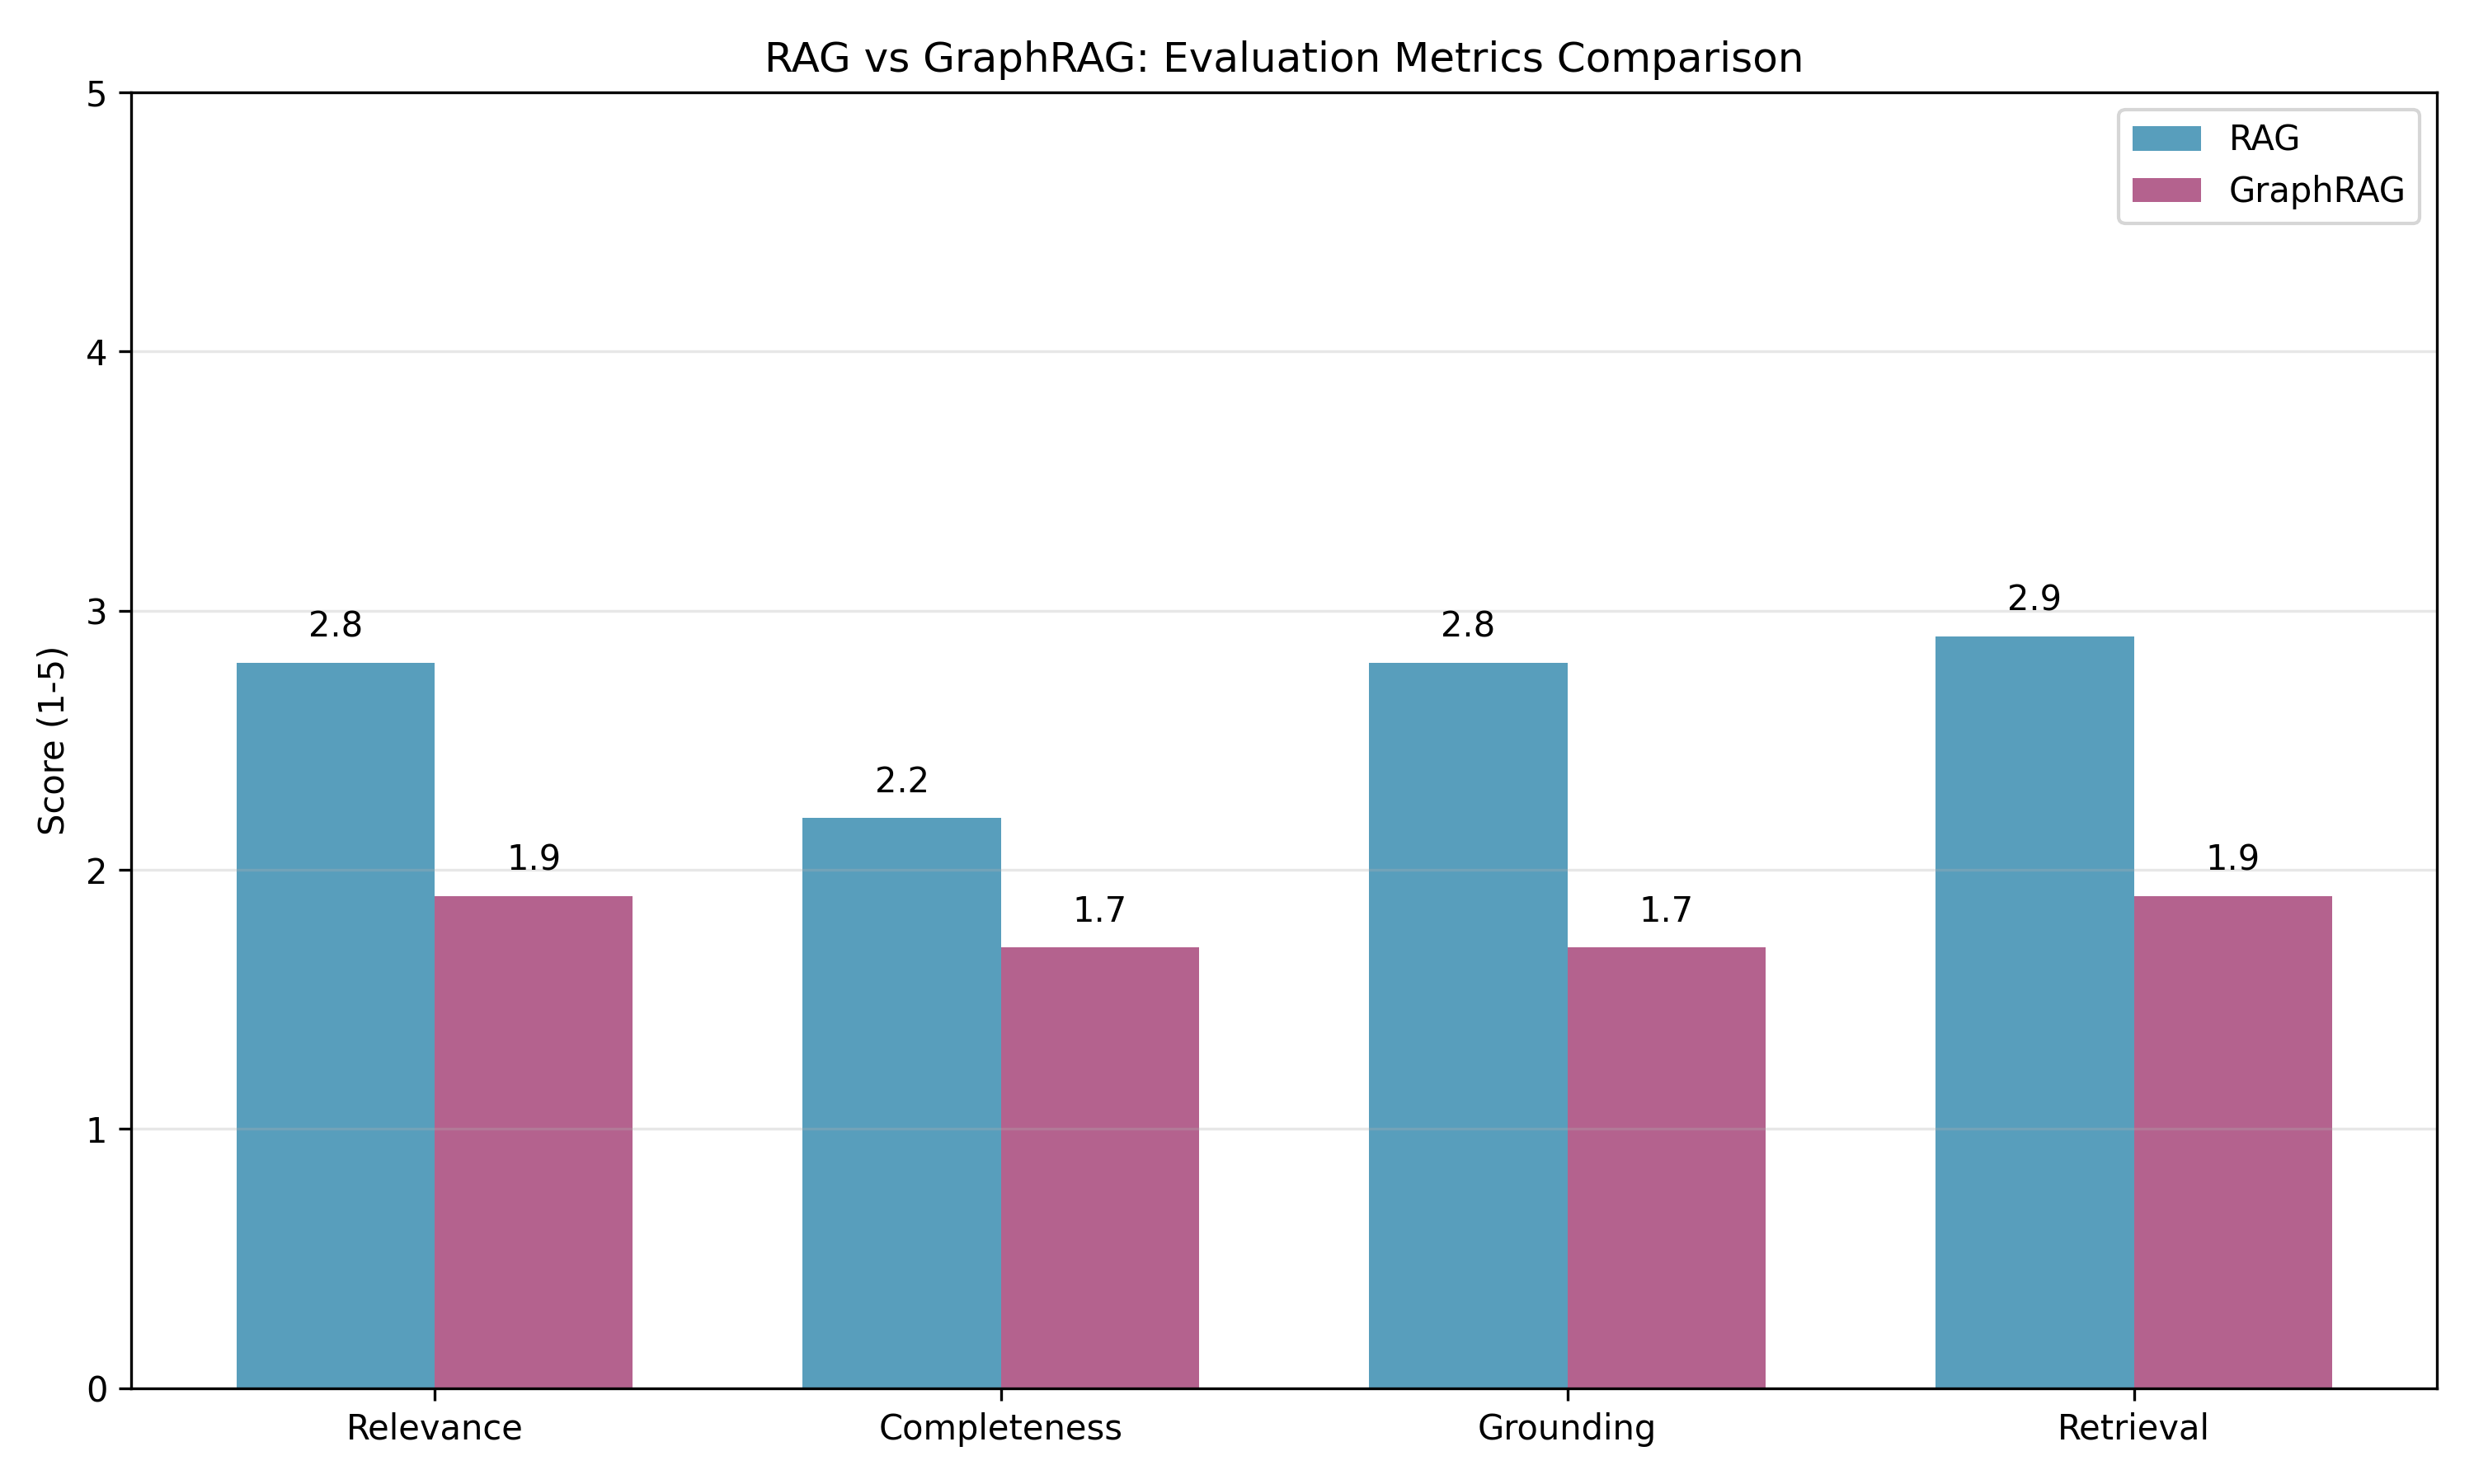
\includegraphics[width=0.48\textwidth]{figures/metrics_comparison.png}
\caption{RAG vs GraphRAG: Evaluation Metrics Comparison}
\label{fig:metrics}
\end{figure}

\begin{figure}[htbp]
\centering
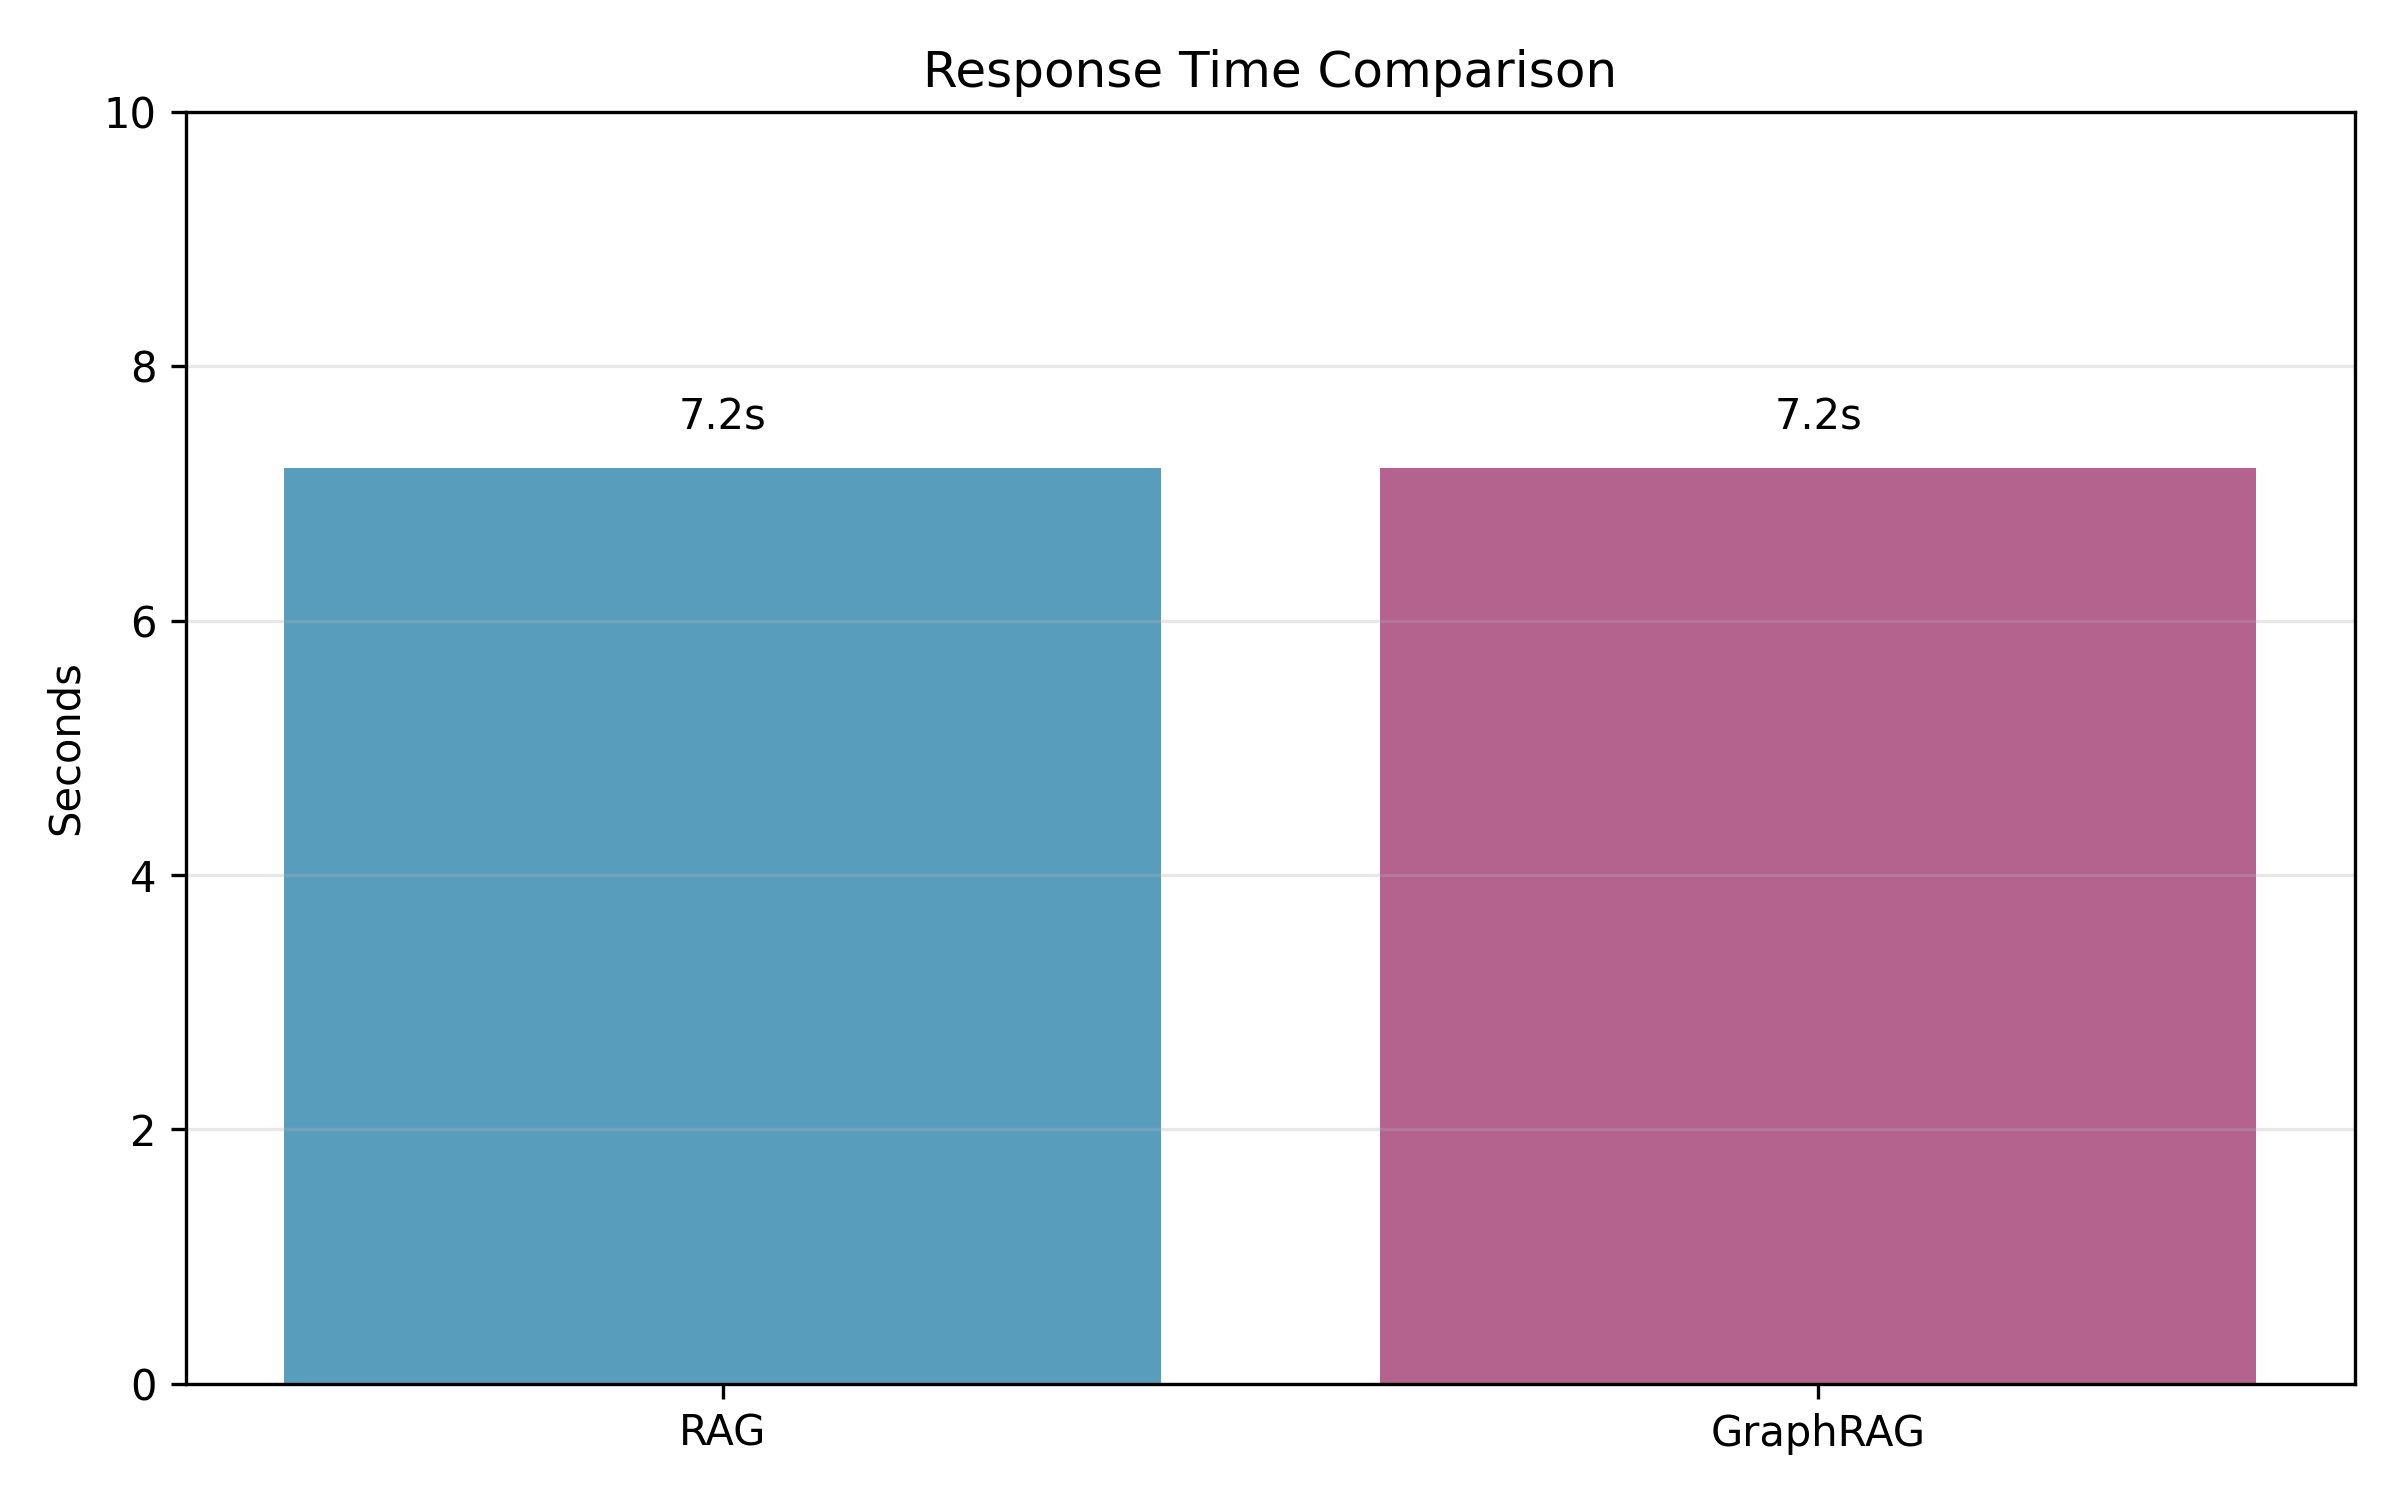
\includegraphics[width=0.48\textwidth]{figures/response_time.png}
\caption{Response Time Comparison: RAG vs GraphRAG}
\label{fig:time}
\end{figure}

\begin{figure}[htbp]
\centering
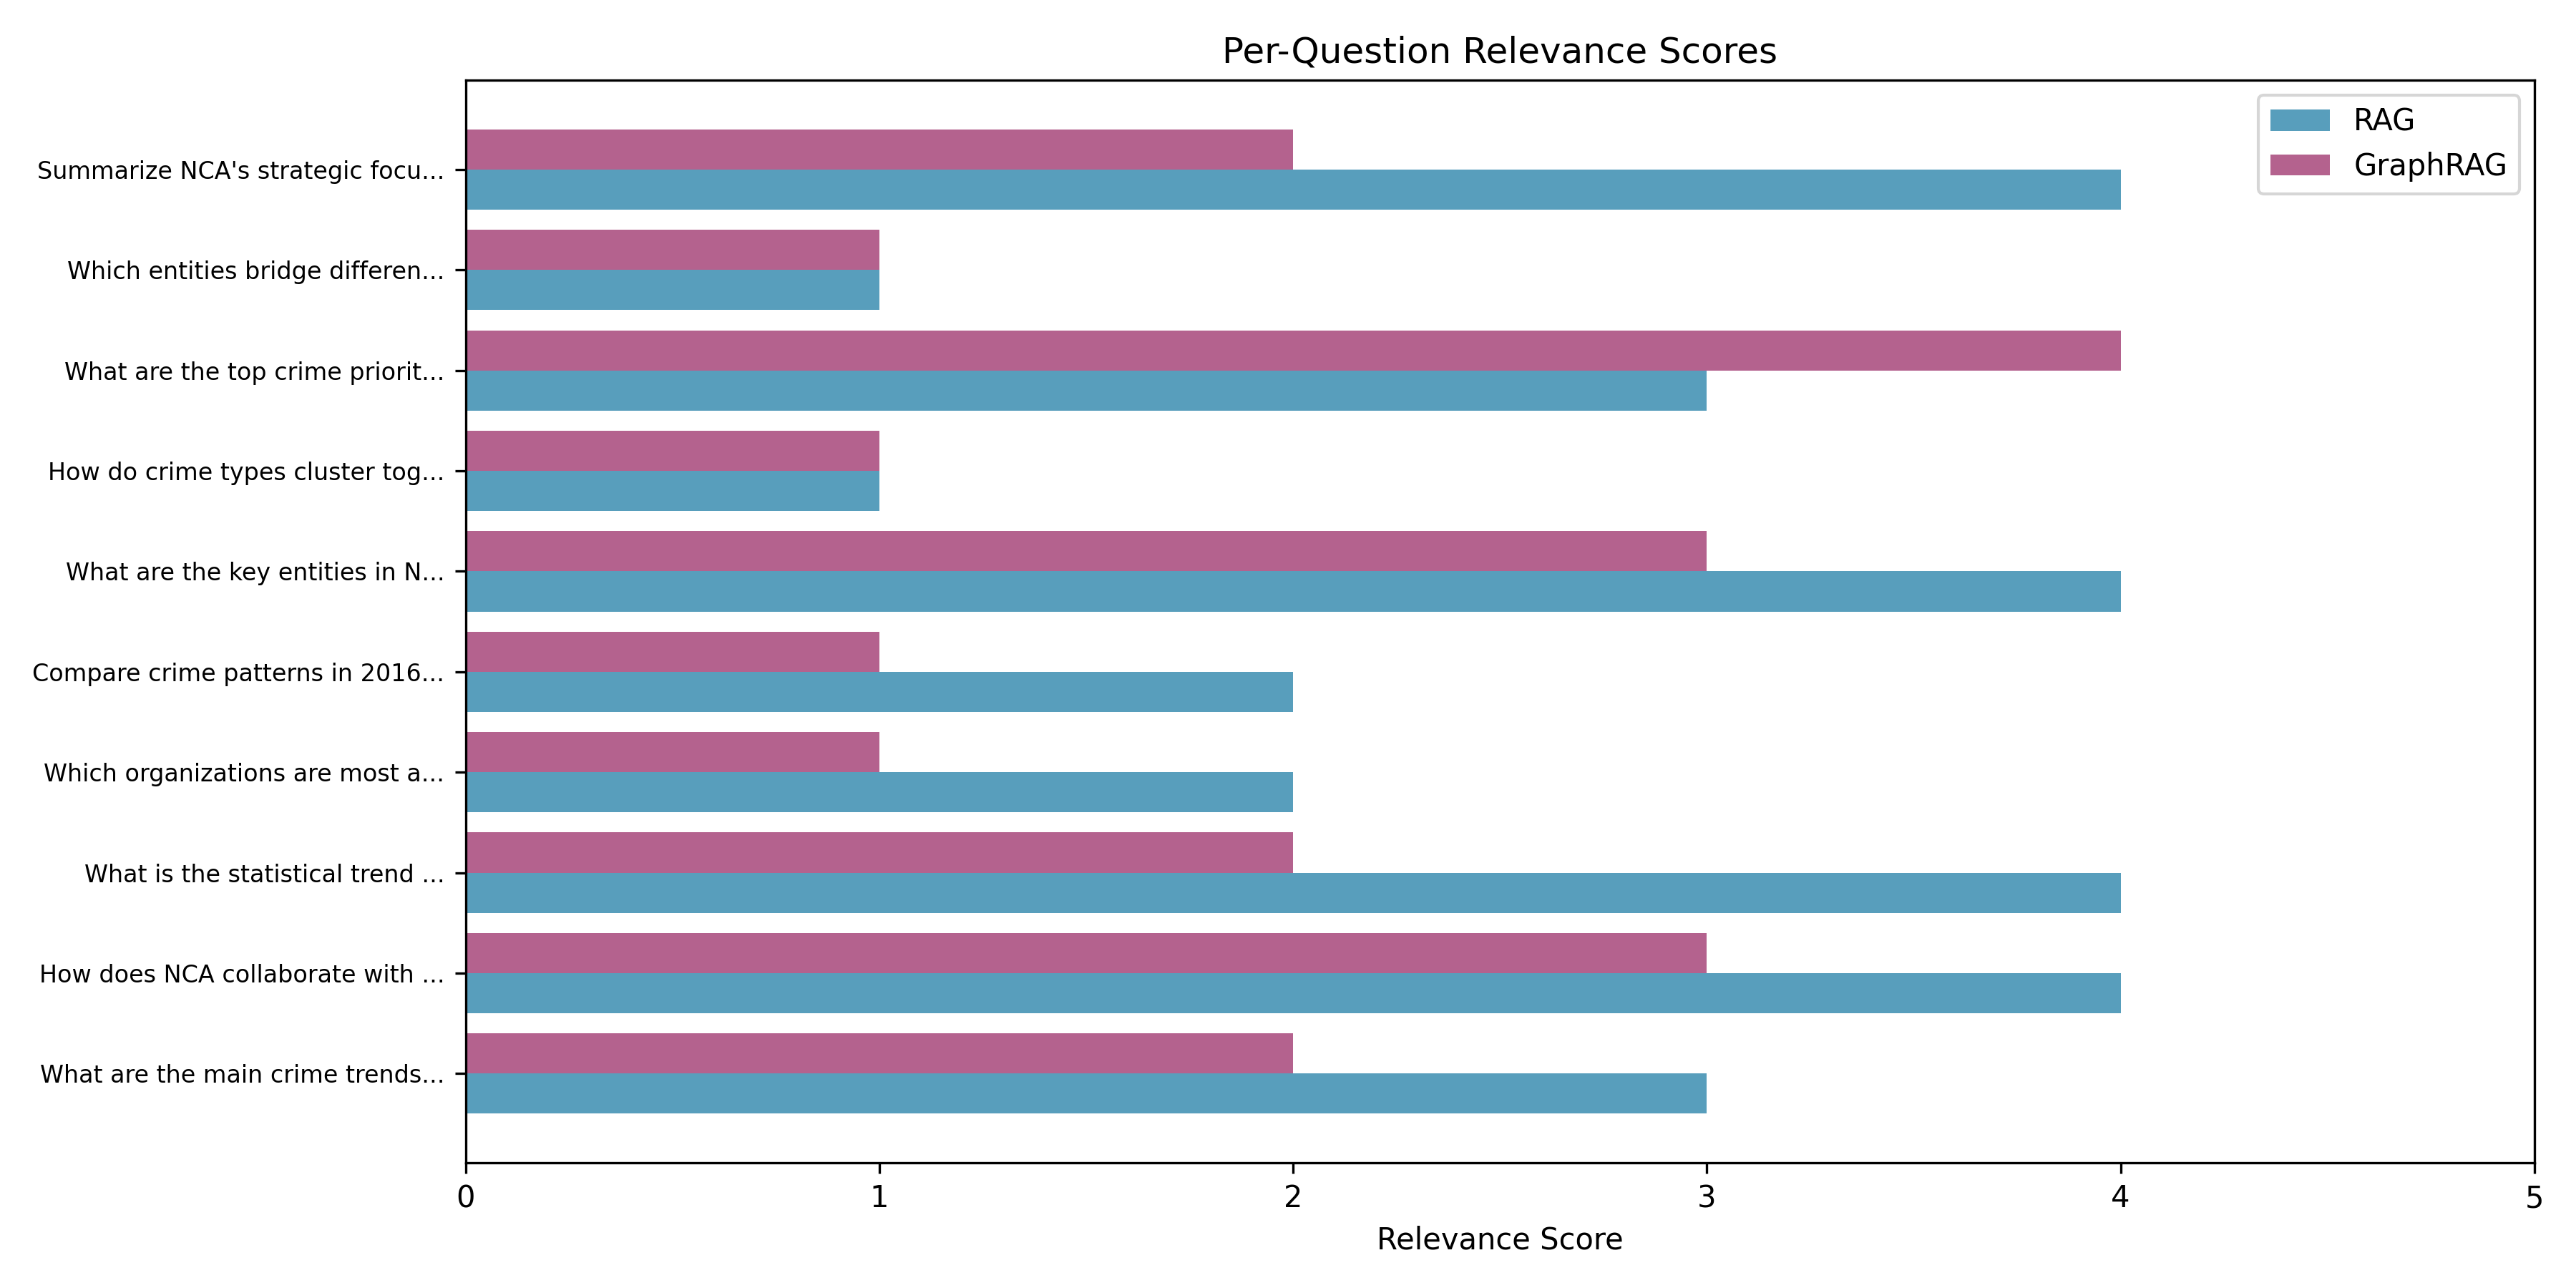
\includegraphics[width=0.48\textwidth]{figures/question_scores.png}
\caption{Per-Question Relevance Scores}
\label{fig:scores}
\end{figure}

\begin{figure}[htbp]
\centering
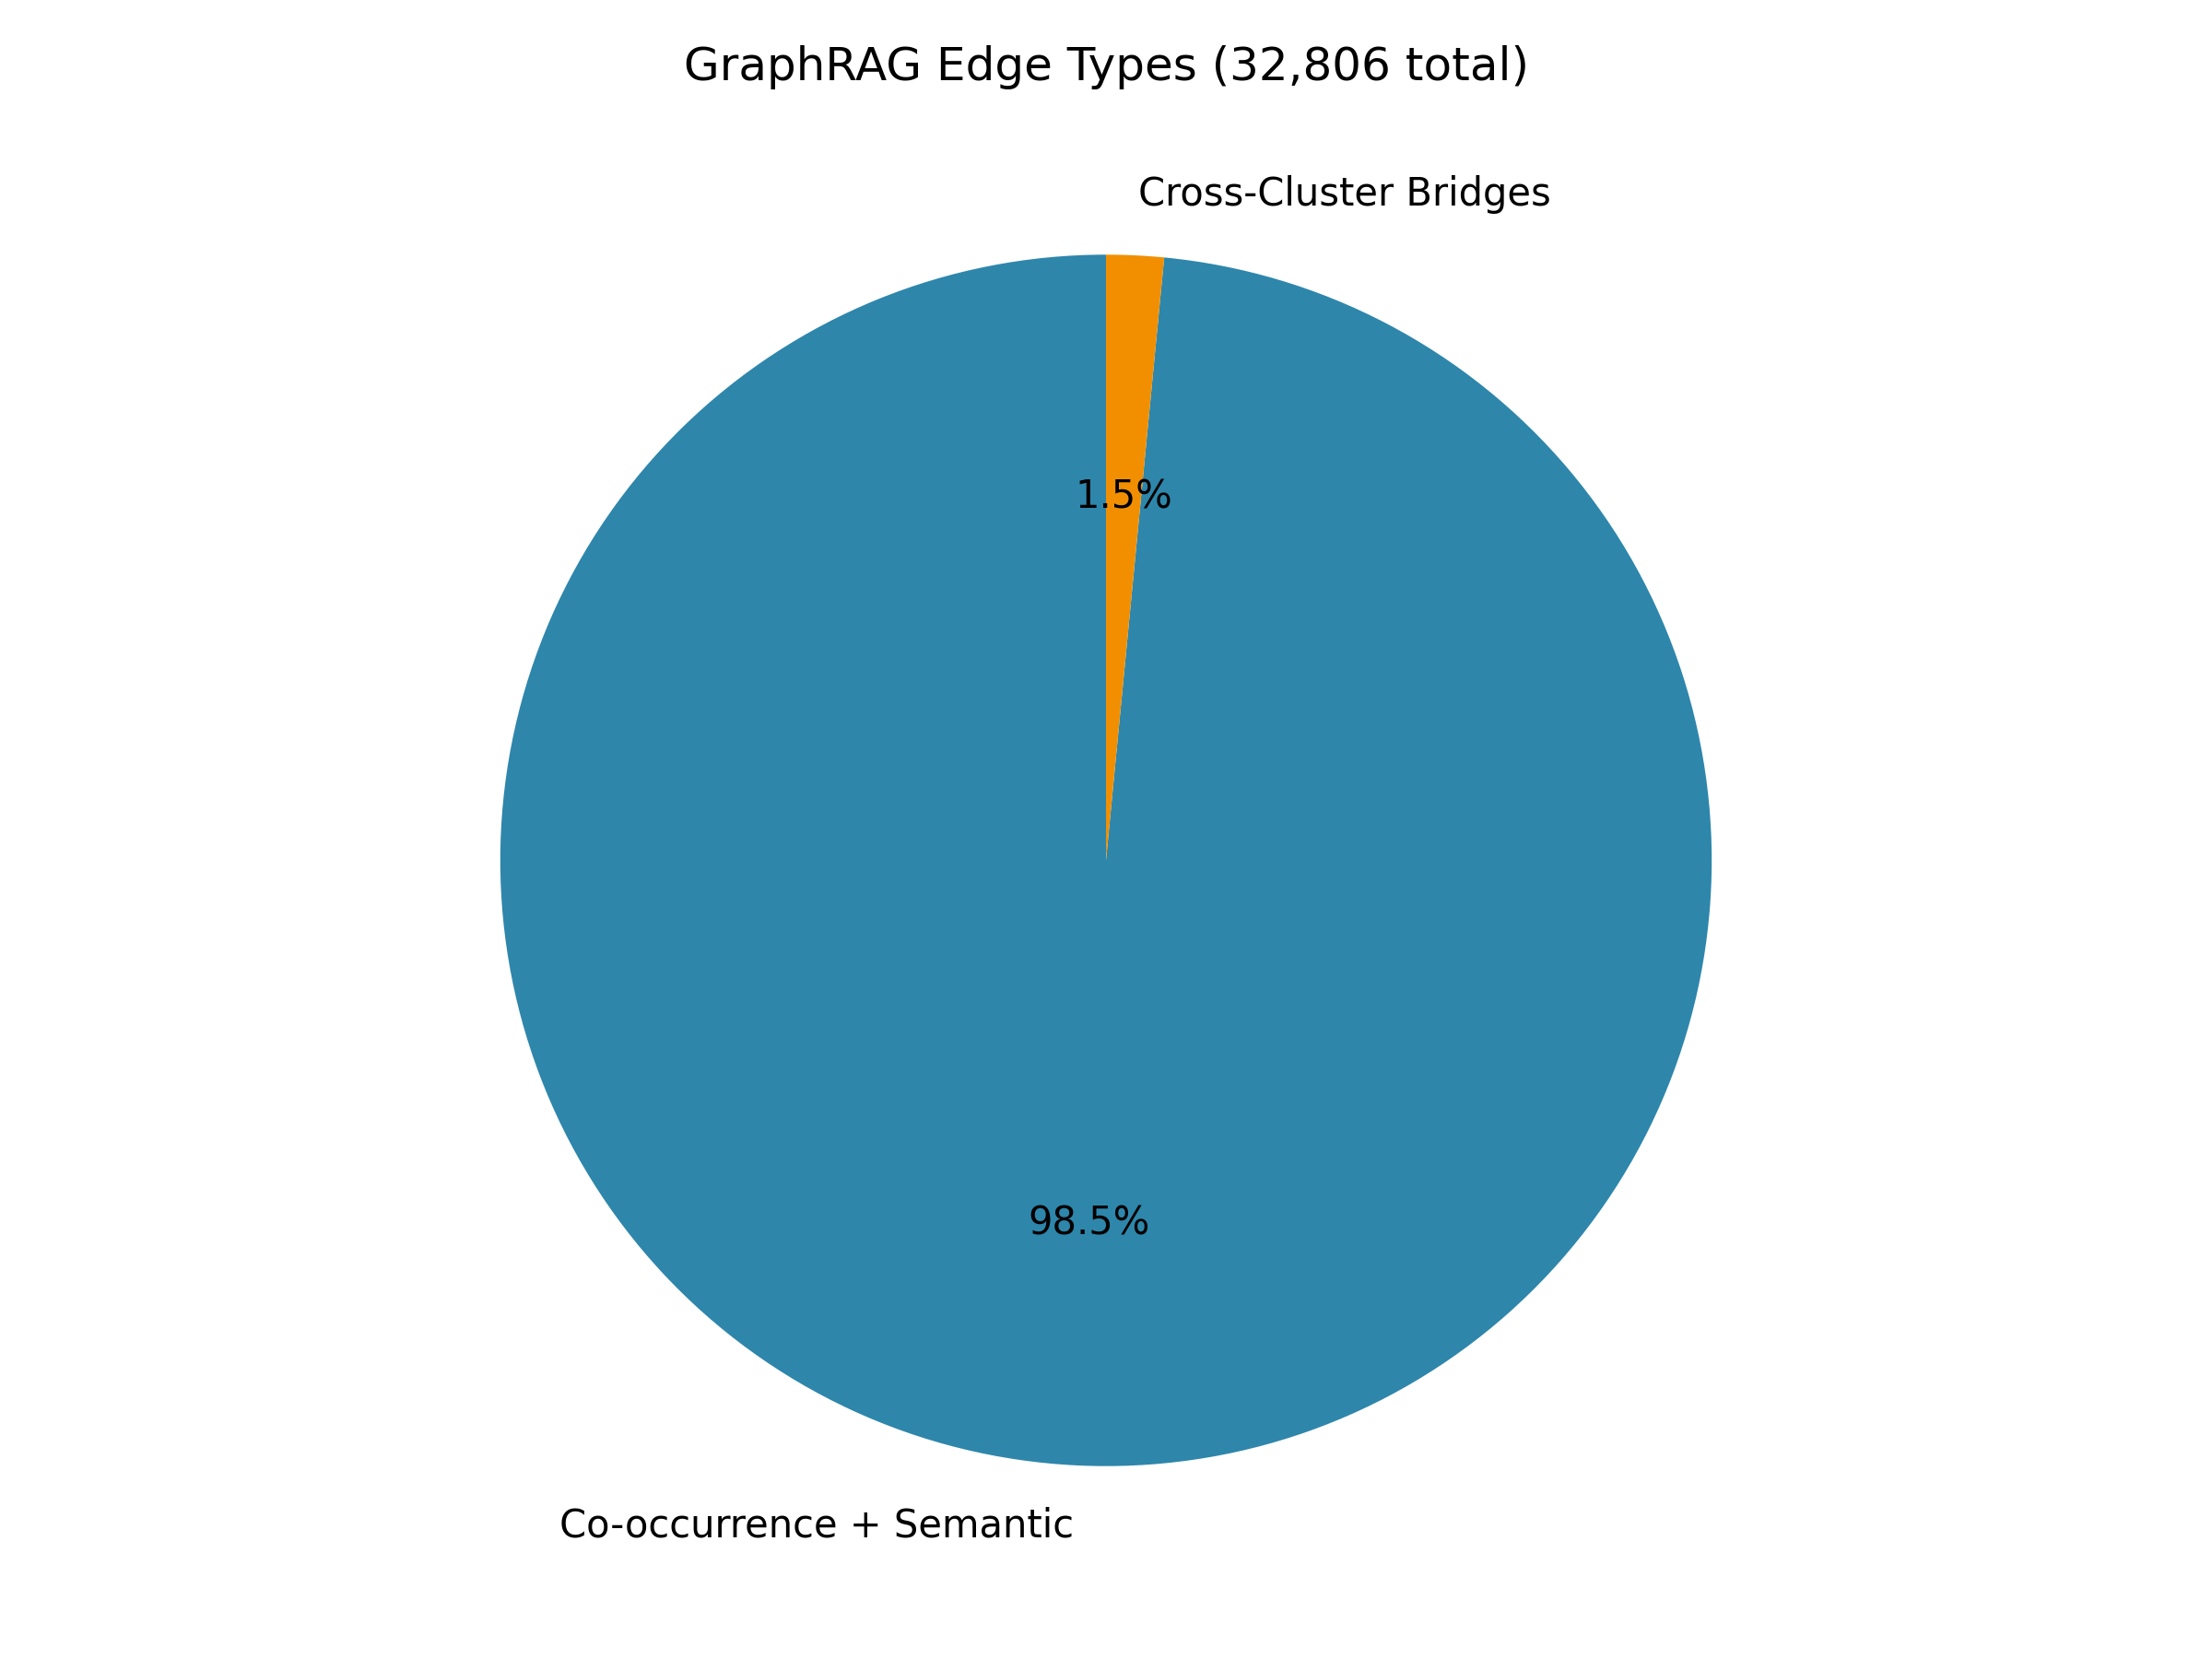
\includegraphics[width=0.48\textwidth]{figures/graph_structure.png}
\caption{GraphRAG Edge Types (32,806 total)}
\label{fig:structure}
\end{figure}

\textbf{Surprising Finding}: Contrary to our hypothesis, RAG outperformed GraphRAG across all metrics. Analysis reveals that GraphRAG's current implementation suffers from:
\begin{itemize}
\item Generic LLM-generated answers not leveraging graph structure effectively
\item Hallucinated content (e.g., claiming "crimes increased 2016-2023" without data)
\item Poor entity-to-chunk mapping, missing relevant context
\end{itemize}

\subsection{Qualitative Comparison}
Table \ref{tab:qa} shows sample question-answer pairs. While GraphRAG should theoretically provide broader context by traversing entity relationships, RAG's direct chunk retrieval proved more reliable for this dataset size.

\begin{table*}[htbp]
\caption{Sample Q\&A Comparison (Excerpts)}
\label{tab:qa}
\centering
\footnotesize
\begin{tabular}{|p{2cm}|p{5cm}|p{5cm}|}
\hline
\textbf{Question} & \textbf{RAG Answer} & \textbf{GraphRAG Answer} \\
\hline
What are main crime trends 2016-2023? & "from church roofs increased in 2022 by 6.8\%..." & "increase in violent crimes such as assault and robbery..." (generic, less grounded) \\
\hline
NCA collaboration? & "NCA-CEOP: Call for Partnerships..." & "NCA invites interested parties..." (repetitive, poor context use) \\
\hline
Human trafficking trends? & "number of potential victims... broadly stable" & "steadily increasing" (contradicts source data) \\
\hline
\end{tabular}
\end{table*}

\subsection{Knowledge Graph Visualization}
Figure \ref{fig:graph} shows the D3.js visualization of the GraphRAG knowledge graph (30\% sample: 3,125 nodes, 3,300+ edges). Pink edges represent \texttt{SEMANTIC\_SIMILAR} connections, gray edges are co-occurrence.

\begin{figure}[htbp]
\centering
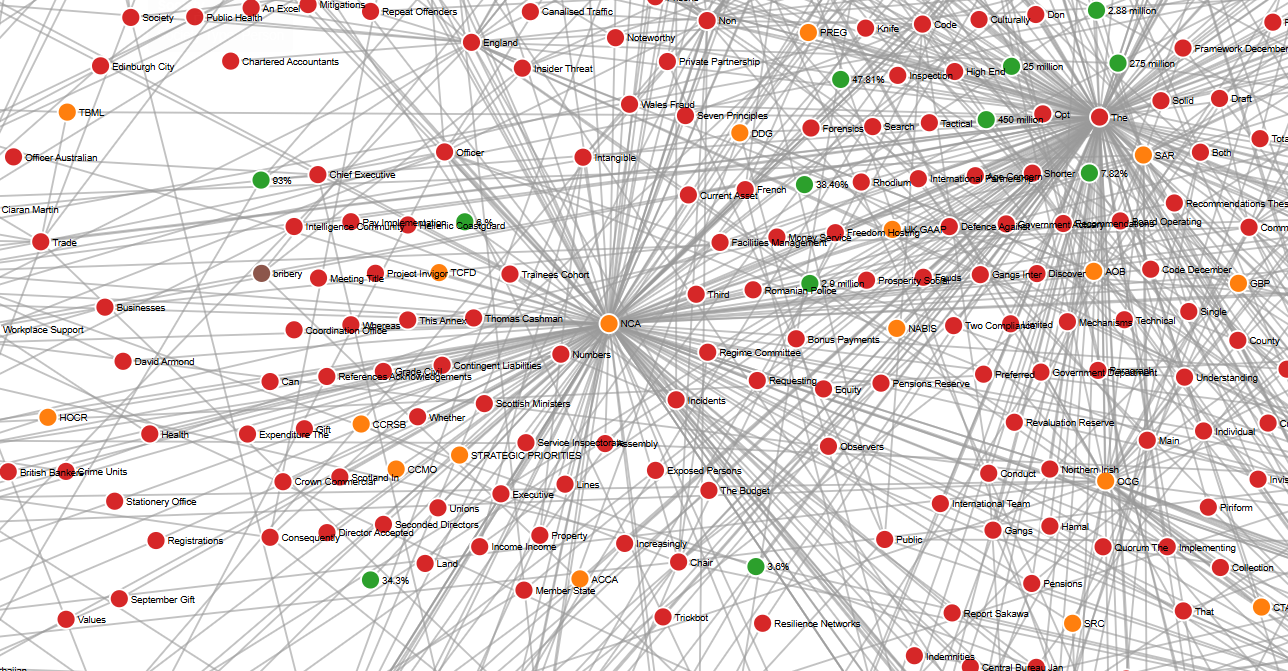
\includegraphics[width=0.45\textwidth]{figures/graph_30percent_screenshot.png}
\caption{GraphRAG Knowledge Graph Visualization (30\% Sample)}
\label{fig:graph}
\end{figure}

\section{Discussion}
\subsection{Key Findings}
Contrary to our hypothesis, \textbf{RAG outperformed GraphRAG} across all metrics (Table \ref{tab:metrics}). RAG achieved higher relevance (2.8 vs 1.9), completeness (2.2 vs 1.7), and grounding (2.8 vs 1.7).

Analysis reveals GraphRAG's current limitations:
\begin{itemize}
\item \textbf{Poor Context Utilization}: Generated answers often ignore graph structure, producing generic LLM responses
\item \textbf{Hallucination}: Claims like "crimes steadily increasing" when source data shows "broadly stable"
\item \textbf{Entity Mapping Issues}: Graph traversal retrieves entities but fails to connect them to relevant text chunks
\end{itemize}

Rule-based extraction proved superior to LLM-based methods (avoids garbage entity names like "entity1"), but the graph construction alone is insufficient without improved query-time integration.

\subsection{Why RAG Succeeded}
\begin{itemize}
\item Direct chunk retrieval ensures answers are grounded in source material
\item Simpler pipeline with fewer failure points
\item ChromaDB's dense retrieval effectively finds relevant context for the 1,529-chunk dataset
\end{itemize}

\subsection{GraphRAG Improvement Needs}
For GraphRAG to fulfill its promise, future work must:
\begin{enumerate}
\item Improve entity-to-chunk mapping (current BFS traversal insufficient)
\item Implement community summarization (Edge et al.'s approach) for global queries
\item Add re-ranking of graph-retrieved context before LLM generation
\item Expand dataset (155 PDFs insufficient for graph advantages to emerge)
\end{enumerate}

\subsection{Challenges}
\begin{itemize}
\item \textbf{Ollama Timeout}: Mistral 7B required 120s timeout for longer generations
\item \textbf{Metrics Collection}: LLM-as-judge failed; manual scoring used
\end{itemize}

\subsection{Limitations}
\begin{itemize}
\item Small dataset (155 PDFs) limits graph connectivity and generalizability
\item Manual metrics scoring introduces subjectivity
\item GraphRAG query implementation requires significant refinement
\end{itemize}

\section{Conclusion}
This comparative analysis reveals that \textbf{RAG outperformed GraphRAG} for the current dataset and implementation. While GraphRAG's knowledge graph (10,417 nodes, 32,806 edges) demonstrates technical sophistication, the query pipeline fails to leverage graph structure effectively. RAG's simplicity and direct chunk retrieval proved more reliable for global sensemaking questions on this dataset. Future work must focus on improving GraphRAG's query-time context integration and expanding the dataset to realize its theoretical advantages.

\section*{Acknowledgment}
We thank the UK National Crime Agency for public access to their documents.

\bibliographystyle{IEEEtran}
\bibliography{references}

\end{document}